\subsection{A fact about our formulas}\label{ss:fact}

We reprint two statement proven in \cite{medina2023fast_sq}.
For $U \in \P_{n-i}^n$ we write $\bar u \notin U$ if $\bar u \in \{0, \dots, n\} \setminus U$.
We simplify notation writing $\bar u.U$ instead of $\{\bar u\} \union U$ if $\bar u \notin U$ and $U \setminus u$ instead of $U \setminus \{u\}$ if $u \in U$.

\begin{proposition}\label{p:fact}
	For $i,n \in \N$ with $i < n$ we have:
	\[
	\canonical_i \bd \, [n] =
	\sum_{\mathclap{U \in \P_{n-i}^n}} \
	\left(\
	\sum_{\mathclap{u \in U^1}} u.U^0 \ot U^1 +
	\sum_{\mathclap{u \in U^0}} U^0 \ot u.U^1
	\right).
	\]
\end{proposition}

\anibal{Missing the other one}

\newpage
\anibal{Below the old}
\subsection{Preparing the induction step}\label{ss:preparing}

We will prove two statements that are key to prove the induction step of the argument establishing our main result.

\begin{notation*}
	Given a function $\xi \colon \P_{n-i}^n \to \F$ we denote by $\barxi \colon \P_{n-i}^n \to \F$ the function defined by the condition $\barxi(U) \neq \xi(U) \text{ for all } U \in \P_{n-i}^n$.
	We will simplify notation writing $U^\xi$ and $U^{\barxi}$ instead of $U^{\xi(U)}$ and $U^{\barxi(U)}$.
\end{notation*}

\begin{lemma}\label{l:first nail}
	Let $\big\{ \triangle_i [n] \big\}_{i,n\in\N}$ be a free and non-zero simplicial \mbox{cup-$i$} construction and $i,n \in \N$ with $i \leq n-2$.
	If there is a function $\xi \colon \P_{n-i}^n \to \F$ with
	\begin{equation}\label{e:xi and barxi}
		\triangle_i [n] =
		\sum_{\mathclap{U \in \P_{n-i}^n}} U^{\xi} \ot U^{\barxi}
	\end{equation}
	and either
	\[
	\triangle_i [n-1] = \canonical_i [n-1]
	\quad \text{or} \quad
	\triangle_i [n-1] = T\canonical_i [n-1],
	\]
	then $\xi$ is constant, i.e.,
	\[
	\triangle_i [n] = \canonical_i [n]
	\quad \text{or} \quad
	\triangle_i [n] = T \canonical_i [n].
	\]
\end{lemma}

\begin{proof}
	Let us assume $\triangle_i [n-1] = \canonical_i [n-1]$.
	The other case is proven analogously.
	Applying the boundary of $\cP(\simplex^n)^{\ot 2}$ -- \cref{e:boundary of P} -- to \cref{e:xi and barxi} gives
	\begin{align*}
		\bd \triangle_i [n] & =
		\sum_{\mathclap{U \in \P_{n-i}^n}} \
		\left(\
		\sum_{\mathclap{\bar u \notin U}} \bar u.U^\xi \ot U^\barxi +
		\sum_{\mathclap{\bar u \notin U}} U^\xi \ot \bar u.U^\barxi
		\right) \\ & +
		\sum_{\mathclap{U \in \P_{n-i}^n}} \
		\left(\
		\sum_{\mathclap{u \in U^\barxi}} u.U^\xi \ot U^\barxi +
		\sum_{\mathclap{u \in U^{\xi}}} U^\xi \ot u.U^\barxi
		\right).
	\end{align*}
	Combining our assumption and \cref{p:fact} gives
	\[
	\triangle_i \bd \, [n] =
	\canonical_i \bd \, [n] =
	\sum_{\mathclap{U \in \P_{n-i}^n}} \
	\left(\
	\sum_{\mathclap{u \in U^1}} u.U^0 \ot U^1 +
	\sum_{\mathclap{u \in U^0}} U^0 \ot u.U^1
	\right).
	\]
	Adding this last two identities together gives
	\begin{align}
		(1+T) \triangle_{i-1} [n] &=
		\bd \triangle_i [n] + \triangle_i \bd \, [n] \\ &=
		\label{e:top} \sum_{\mathclap{U \in \P_{n-i}^n}} \
		\left(\
		\sum_{\mathclap{\bar u \notin U}} \bar u.U^\xi \ot U^\barxi +
		\sum_{\mathclap{\bar u \notin U}} U^\xi \ot \bar u.U^\barxi
		\right) \\ &+ \,
		\label{e:bottom} (1+T) \sum_{\mathclap{\substack{U \in \P_{n-i}^n \\ \xi(U) \neq 0}}} \
		\left(\
		\sum_{\mathclap{u \in U^1}} u.U^0 \ot U^1 +
		\sum_{\mathclap{u \in U^0}} U^0 \ot u.U^1
		\right).
	\end{align}
	We will use \cref{l:kernel of sxs} to show that summand \eqref{e:top} is in $\ker \cP(\sigma_j)^{\ot 2}$ for every codegeneracy $\sigma_j \colon [n] \to [n-1]$.
	Consider $U \in \P_{n-i}^n$.
	If $\{j, j+1\} \cap U = \emptyset$ then for every $\bar u \notin U$ we have $\bar u.U^\xi \ot U^\barxi \in \ker \cP(\sigma_j)^{\ot 2}$ and $U^\xi \ot \bar u.U^\barxi \in \ker \cP(\sigma_j)^{\ot 2}$.
	If $\{j, j+1\} \cap U = \{j, j+1\}$ then the same conclusion follows from the fact that $\ind_U(j) = \ind_U(j+1)$.
	If $\{j, j+1\} \cap U = \{j\}$ then $\bar u.U^\xi \ot U^\barxi \in \ker \cP(\sigma_j)^{\ot 2}$ and $U^\xi \ot \bar u.U^\barxi \in \ker \cP(\sigma_j)^{\ot 2}$ for every $\bar u \notin U$ with $\bar u \neq j+1$.
	Furthermore, if $j \in U^\xi$ then $(j+1).U^\xi \ot U^\barxi \in \ker \cP(\sigma_j)^{\ot 2}$ and $U^\xi \ot (j+1).U^\barxi \notin \ker \cP(\sigma_j)^{\ot 2}$.
	An analogous statement holds if $j \in U^\barxi$ and a similar analysis applies to the case $\{j, j+1\} \cap U = \{j+1\}$.
	We will show that the basis elements in \eqref{e:top} that are not in $\ker \cP(\sigma_j)^{\ot 2}$ cancel in pairs after the application of $\cP(\sigma_j)^{\ot 2}$.
	Let $\Gamma_j^\xi \subseteq \P_{n-i}^n$ consists of elements $U$ with $\{j, j+1\} \cap U = \{j\}$ and $j \in U^\xi$.
	Let $\Gamma_{j+1}^\xi$, $\Gamma_j^\barxi$, and $\Gamma_{j+1}^\barxi$ be defined analogously.
	The claim follows from the existence of the bijections $\Gamma_{j}^\xi \cong \Gamma_{j+1}^\xi$ and $\Gamma_{j}^\barxi \cong \Gamma_{j+1}^\barxi$ defined by the assignments $U \mapsto (j+1).\big( U \setminus \{j\} \big)$ and $U \mapsto j.\big( U \setminus \{j+1\} \big)$, since two summands related by one of these bijections are sent to the same element by $\cP(\sigma_j)^{\ot 2}$.

	We will impose conditions on summand \eqref{e:bottom} following an analysis similar to the one just given.
	Notice that $(1+T)$ commutes with $\cP(\sigma_j)^{\ot 2}$ and that the only basis elements in \eqref{e:bottom} not in $\ker \cP(\sigma_j)^{\ot 2}$ are associated to pairs $(U, u)$ with $\xi(U) \neq 0$ and $u = j$ or $ u = j+1$.
	Let $\Lambda_{j}^0$ be the subset of $\{U \in \P_{n-i}^n \mid \xi(U) \neq 0\}$ consisting of sets $U$ with $j \in U^0$ and $j+1 \notin U$.
	We define $\Lambda_{j}^1$, $\Lambda_{j+1}^0$, and $\Lambda_{j+1}^1$ analogously.
	The set $\Lambda_{j \wedge j+1}$ is defined by the conditions $\xi(U) \neq 0$ and $j,j+1 \in U$.

	Observe that the sum
	\[
	\sum_{\mathclap{\Lambda_{j \wedge j+1}}}
	\left(\
	\sum_{u \in U^1} u.U^0 \ot U^1 +
	\sum_{u \in U^0} U^0 \ot u.U^1
	\right)
	\]
	is in $\ker \cP(\sigma_j)^{\ot 2}$ since, given that $\ind_U(j) = \ind_U(j+1)$, the only non-zero summands, which are associated to $(U,j)$ and $(U,j+1)$, cancel each other.
	Therefore, applying $\cP(\sigma_j)^{\ot 2}$ to
	\[
	\sum_{\mathclap{\substack{\P_{n-i}^n \\ \xi(U) \neq 0}}}
	\left(\
	\sum_{u \in U^1} {u.U^0} \ot U^1 +
	\sum_{u \in U^0} {U^0} \ot u.U^1
	\right)
	\]
	yields
	\begin{align*}
		&\sum_{\mathclap{\Lambda_{j}^0}} U^0 \setminus \{j\} \ot U^1	+
		\sum_{\mathclap{\Lambda_{j}^1}} U^0 \ot U^1 \setminus \{j\} \\ +
		&\sum_{\mathclap{\Lambda_{j+1}^0}} U^0 \setminus \{j+1\} \ot U^1 +
		\sum_{\mathclap{\Lambda_{j+1}^1}} U^0 \ot {U^1} \setminus \{j+1\}.
	\end{align*}
	which must be in the kernel of $(1+T)$.
	This implies the existence of an involution $\phi^{(j)}$ of $\Lambda = \Lambda^0_{j} \sqcup \Lambda^1_{j} \sqcup \Lambda^1_{j+1} \sqcup \Lambda^1_{j+1}$ defined by a choice of canceling pairs.
	By the freeness of $\canonical$ and since $i \leq n-2$, this involution has no fixed points.
	It follows that two elements $U$ and $U^\prime$ with $U \cap \{j, j+1\} = U^\prime \cap \{j, j+1\}$ cannot be related by $\phi^{(j)}$ since then $U = U^\prime$.
	Therefore, $\phi^{(j)}(U) = U^\prime$ if and only if $U^\prime = j.(U \setminus \{j+1\})$ or $U^\prime = (j+1).\big( U \setminus \{j+1\} \big)$.
	Recall that by definition $\xi(U) = \xi(U^\prime) \neq 0$.
	This analysis applies to any $j \in \{0, \dots, n\}$ and we introduce a relation in $\P_{n-i}^n$ writing $U \sim U^\prime$ if $U^\prime = j.(U \setminus \{j+1\})$ or $U^\prime = (j+1).\big( U \setminus \{j+1\} \big)$ for some $j$.
	By the previous analysis, if $U \sim U^\prime$ then $\xi(U) = \xi(U^\prime)$.
	Any two elements $V$ and $W$ in $\P_{n-i}^n$ are related by a sequence
	\[
	V \sim \dots \sim W,
	\]
	so $\xi \colon \P_{n-i}^n \to \F$ must be constant as claimed.
\end{proof}

\begin{lemma}\label{l:second nail}
	Let $\big\{ \triangle_i [n] \big\}_{i,n\in\N}$ be a non-zero, irreducible, and free simplicial \mbox{cup-$i$} construction and $i,n \in \N$ with $i \leq n-2$.
	If $\triangle_i [n] = \canonical_i [n]$ or $\triangle_i [n] = T \canonical_i [n]$ then the following implications hold:
	\begin{alignat*}{2}
		&\boxed{\triangle_i [n-1] = \canonical_i [n-1] \kern 7.3pt}\ &\Longrightarrow\
		&\boxed{\triangle_i [n] = \canonical_i [n] \kern 7.3pt} \\
		&\boxed{\triangle_i [n-1] = T \canonical_i [n-1]}\ &\Longrightarrow\
		&\boxed{\triangle_i [n] = T \canonical_i [n]} \ .
	\end{alignat*}
\end{lemma}

\begin{proof}
	We use the convention $\triangle_{-1} [n] = \canonical_{-1} [n] = 0$ for all $n \in \N$.
	We will establish the first of the implications above using a proof by contradiction for which we assume $\triangle_i [n-1] = \canonical_i [n-1]$ and $\triangle_i [n] = T \canonical_i [n]$.
	The second implication is proven analogously.
	We have
	\begin{align*}
		(1+T) \triangle_{i-1}[n] &=
		\bd \triangle_i [n] + \triangle_i \bd \, [n] \\ &=
		\bd T \canonical_i [n] + \canonical_i \bd \, [n] \\ &=
		T \bd \canonical_i [n] + \bd \canonical_i [n] + \bd \canonical_i [n] + \canonical_i \bd \, [n] \\ &=
		(1+T) \bd \canonical_i [n] + (1+T) \canonical_{i-1} [n] \\ &=
		(1+T) \canonical_i \bd \, [n] + (1+T) \canonical_{i-1} [n].
	\end{align*}
	Using \cref{p:fact,l:canonical}, i.e.
	\[
	\begin{split}
		\canonical_i \bd \, [n] &=
		\sum_{\mathclap{U \in \P_{n-i}^n}} \
		\left(\
		\sum_{\mathclap{u \in U^1}} u.U^0 \ot U^1 +
		\sum_{\mathclap{u \in U^0}} U^0 \ot u.U^1
		\right), \\
		\canonical_{i-1} [n] &=
		\sum_{\mathclap{V \in \P_{n-i+1}^n}} V^0 \ot V^1,
	\end{split}
	\]
	we have
	\begin{align*}
		(1+T) \triangle_{i-1}[n] &=
		(1+T) \sum_{\mathclap{U \in \P_{n-i}^n}} \
		\left(\
		\sum_{\mathclap{u \in U^1}} u.U^0 \ot U^1 +
		\sum_{\mathclap{u \in U^0}} U^0 \ot u.U^1
		\right) \\ &+
		(1+T) \sum_{\mathclap{V \in \P_{n-i+1}^n}} V^0 \ot V^1.
	\end{align*}
	By \cref{l:consequence} there are functions $\eta \colon \P_{n-i}^n \to \F$ and $\zeta \colon \P_{n-i+1}^n \to \F$ such that
	\begin{align*}
		\triangle_{i-1}[n] \ &=
		\sum_{\mathclap{U \in \P_{n-i}^n}} \
		\left(\
		\sum_{\mathclap{u \in U^\bareta}} u.U^\eta \ot U^\bareta +
		\sum_{\mathclap{u \in U^\eta}} U^\eta \ot u.U^\bareta
		\right) \\ &+
		\sum_{\mathclap{V \in \P_{n-i+1}^n}} V^\zeta \ot V^\barzeta.
	\end{align*}
	This contradicts the irreducibility of $\big\{ \triangle_i [n] \big\}_{i,n \in \N}$ as expressed in \cref{l:properties}.
\end{proof}

\subsection{Induction step}\label{ss:step}

We prove the induction step of the argument proving our main result.

\begin{figure}
	\centering
	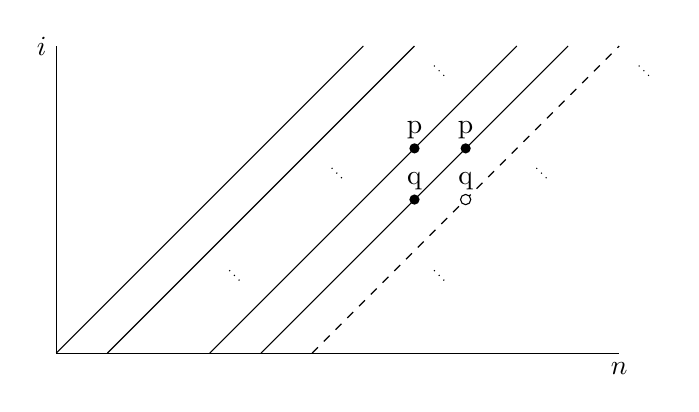
\begin{tikzpicture}[scale = .65]
	\draw (0,0)--(0,6);
	\draw (0,0)--(11,0);
	\draw (0,0)--(6,6);
	\draw (1,0)--(7,6);
	\draw (3,0)--(9,6);
	\draw (4,0)--(10,6);
	\draw[dashed] (5,0)--(11,6);

	\draw[dotted, shorten >=10pt,shorten <=10pt] (3,2)--(4,1);
	\draw[dotted, shorten >=10pt,shorten <=10pt] (5,4)--(6,3);
	\draw[dotted, shorten >=10pt,shorten <=10pt] (7,6)--(8,5);

	\fill (7,4) circle (0.1);
	\fill (8,4) circle (0.1);
	\fill (7,3) circle (0.1);
	\fill[white] (8,3) circle (0.1);
	\draw (8,3) circle (0.1);

	\node[above] at (7,4) {p};
	\node[above] at (8,4) {p};
	\node[above] at (7,3) {q};
	\node[above] at (8,3) {q};

	\draw[dotted, shorten >=10pt,shorten <=10pt] (7,2)--(8,1);
	\draw[dotted, shorten >=10pt,shorten <=10pt] (9,4)--(10,3);
	\draw[dotted, shorten >=10pt,shorten <=10pt] (11,6)--(12,5);

	\node[below] at (11,0) {$n$};
	\node[left] at (0,6) {$i$};
	\end{tikzpicture}
	\caption{Representation of the implication in \cref{l:induction step} serving as the induction step in the proof of \cref{t:main}.}
	\label{f:induction step}
\end{figure}

\begin{lemma}\label{l:induction step}
	Let $\big\{ \triangle_i [n] \big\}_{i,n\in\N}$ be a free non-zero and irreducible simplicial \mbox{cup-$i$} construction.
	Let $\big\{ \p(i,n) \big\}_{i,n \in \N}$ and $\big\{ \q(i,n) \big\}_{i,n \in \N}$ each be one of the following two families of propositions:
	\[
	\big\{ \triangle_i [n] = \canonical_ i [n] \big\}_{i,n \in \N}
	\quad \text{or} \quad
	\big\{ \triangle_i [n] = T \canonical_ i [n] \big\}_{i,n \in \N} \ .
	\]
	For all $i,n \in \N$ with $i \leq n-2$ the following implication holds:
	\[
	\boxed{\p(i+1,n) \wedge \p(i+1,n-1) \wedge \q(i,n-1)}\ \Longrightarrow\ \boxed{\q(i,n)}
	\]
\end{lemma}

\begin{proof}
	Let both $\big\{ \p(i,n) \big\}_{i,n\in\N}$ and $\big\{ \q(i,n) \big\}_{i,n\in\N}$ be the family $\big\{ \triangle_i [n] = \canonical_i [n] \big\}_{i,n \in \N}$.
	The other three combinations are treated analogously.

	From $\p(i+1,n)$ and $\p(i+1,n-1)$ we have
	\[
	\bd \triangle_{i+1} [n] + \triangle_{i+1} \bd \, [n] =
	\bd \canonical_{i+1} [n] + \canonical_{i+1} \bd \, [n]
	\]
	or, equivalently,
	\begin{align*}
		(1+T) \triangle_i [n] =
		(1+T) \canonical_i [n] \defeq
		(1+T) \sum_{\mathclap{U \in \P_{n-i}^n}} {U^0} \ot {U^1}
	\end{align*}
	\cref{l:consequence} implies the existence of a function $\xi \colon \rP_{n-i}^n \to \Ftwo$ such that
	\[
	\triangle_i [n] =
	\sum_{\mathclap{U \in \P_{n-i}^n}} U^\xi \ot U^\barxi.
	\]
	\cref{l:first nail} implies, using $\q(i,n-1)$, that
	\[
	\triangle_i [n] = \canonical_i [n]
	\quad \text{or} \quad
	\triangle_i [n] = T \canonical_i [n].
	\]
	Finally, \cref{l:second nail} implies $\triangle_i [n] = \canonical_i [n]$, i.e., $\q(i,n)$.
\end{proof}

\subsection{Complete proof}\label{ss:proof}

We now present the proof of our main result.

\begin{proof}[Proof of \cref{t:main}]
	Let $\big\{ \triangle_i [n] \big\}_{i,n\in\N}$ be a non-zero, irreducible, and free simplicial \mbox{cup-$i$} construction.
	We will use an induction argument over $k = n-i$ to show that for each $i \in \N$ either $\triangle_i [n] = \canonical_i [n]$ or
	$\triangle_i [n] = T \canonical_i [n]$ for all $n \in \N$.
	By \cref{l:special case one} $\triangle_i [n] = \canonical_i [n]$ and $\triangle_i [n] = T \canonical_i [n]$ for $k \leq 0$.
	By \cref{l:special case two} $\triangle_i [n] = \canonical_i [n]$ or $\triangle_i [n] = T \canonical_i [n]$ for $r = 1$.
	This serves as the base case of the induction and \cref{l:induction step} as the induction step (\cref{f:induction step}).
\end{proof}


\newpage
ERASERAESAE
\begin{proposition}
	Let $\triangle$ be a cup-$i$ construction and $i_0$ and $n_0$ positive integers.
	If
	\[
	\widetilde\triangle_i[n] =
	\begin{cases}
		T\triangle_{i}[n] & i = i_0,n=n_0, \\
		\big(\triangle_{i} + \bd \triangle_{i+1}\big)[n] & 0 < i_0-i =n-n_0, \\
		\triangle_{i}[n] & \text{otherwise}.
	\end{cases}
	%	\begin{cases}
		%		T\triangle_{i_0}[n_0] & i = i_0 \text{ and } n=n_0, \\
		%		\big(\triangle_{i_0-\ell} + \bd \triangle_{i_0-\ell+1}\big)[n_0+\ell] & i = i_0-\ell \text{ and } n=n_0+\ell, \\
		%		\triangle_{i}[n] & \text{otherwise}.
		%	\end{cases}
	\]
	Then $\widetilde\triangle = \set[\big]{\widetilde\triangle_i[n]}_{i,n}$ is a cup-$i$ construction.
\end{proposition}

\begin{proof}
	We need to verify that for each pair $i,n$ the identity
	\[
	\big(\bd \widetilde\triangle_{i} + \widetilde\triangle_{i}\bd\big)[n] =
	(1+T) \widetilde\triangle_{i-1}[n]
	\]
	holds, knowing it does so for $\triangle$.
	We will split the proof into four cases
	\[
	i < i_0 \quad;\quad i = i_0 \quad;\quad i = i_0+1 \quad;\quad i > i_0+1.
	\]
	If $i > i_0+1$ the identity on $\widetilde\triangle$ reduces to that for $\triangle$.
	Let $i = i_0+1$, if $n \neq n_0$ the same is true, whereas if $n = n_0$ we have
	\begin{align*}
		\big(\bd \widetilde\triangle_{i_0+1} + \widetilde\triangle_{i_0+1} \bd\big) &=
		\big(\bd \triangle_{i_0+1} + \triangle_{i_0+1} \bd\big) \\ &=
		(1+T)\triangle_{i_0} \\ &=
		(1+T)T\triangle_{i_0} \\ &=
		(1+T)\widetilde\triangle_{i_0}.
	\end{align*}
	For $i = i_0$ there are two values of $n$ for which the identity is not immediate.
	For $n = n_0+1$ we have
	\begin{align*}
		\big(\bd \widetilde\triangle_{i_0} + \widetilde\triangle_{i_0} \bd\big) &=
		\big(\bd \triangle_{i_0} + T\triangle_{i_0} \bd\big) \\ &=
		\big((1+T)\bd\triangle_{i_0} + T(\bd\triangle_{i_0} + \triangle_{i_0}\bd)\big) \\ &=
		(1+T)\big(\bd\triangle_{i_0} + \triangle_{i_0-1}\big) \\ &=
		(1+T)\widetilde\triangle_{i_0-1},
	\end{align*}
	and for $n = n_0$ we have
	\begin{align*}
		\big(\bd \widetilde\triangle_{i_0} + \widetilde\triangle_{i_0} \bd\big) &=
		\big(\bd T \triangle_{i_0} + \triangle_{i_0} \bd\big) \\ &=
		\big((1+T)\bd\triangle_{i_0} + \bd\triangle_{i_0} + \triangle_{i_0}\bd\big) \\ &=
		(1+T)\big(\bd\triangle_{i_0} + \triangle_{i_0-1}\big) \\ &=
		(1+T)\widetilde\triangle_{i_0-1}.
	\end{align*}
	Let us assume that $i < i_0$ and let $i = i_0 - \ell$ for some positive integer $\ell$.
	There are two values of $n$ for which the identity in $\widetilde\triangle$ that do not reduce to those in $\triangle$.
	For $n = n_0+\ell$ we have
	\begin{align*}
		\big(\bd\widetilde\triangle_{i_0-\ell} + \widetilde\triangle_{i_0-\ell} \bd\big) &=
		\big(\bd\triangle_{i_0-\ell} + \bd\bd\triangle_{i_0-\ell+1} + \triangle_{i_0-\ell} \bd\big) \\ &=
		(1+T)\triangle_{i_0-\ell-1} \\ &=
		(1+T)\widetilde\triangle_{i_0-\ell-1},
	\end{align*}
	and for $n = n_0+\ell+1$ we have
	\begin{align*}
		\big(\bd \widetilde\triangle_{i_0-\ell} + \widetilde\triangle_{i_0-\ell} \bd\big) &=
		\big(\bd \triangle_{i_0-\ell} + \triangle_{i_0-\ell}\bd + \bd\triangle_{i_0-\ell+1}\bd\big) \\ &=
		(1+T)\big(\triangle_{i_0-\ell-1} + \bd\triangle_{i_0-\ell}\big) \\ &=
		(1+T)\big(\triangle_{i_0-(\ell+1)} + \bd\triangle_{i_0-(\ell+1)+1}\big) \\ &=
		(1+T)\widetilde\triangle_{i_0-\ell-1}.\qedhere
	\end{align*}

	\begin{example*}
		If $n_0-i_0$
	\end{example*}
	%	\noindent \underline{$i_0-\ell+1,n_0+\ell-1$}:DONE
	%	\begin{align*}
		%		\big(\bd\widetilde\triangle_{i_0-\ell+1} + \widetilde\triangle_{i_0-\ell+1} \bd\big) &=
		%		\big(\bd\triangle_{i_0-\ell+1} + \bd\bd\triangle_{i_0-\ell+2} + \triangle_{i_0-\ell+1} \bd\big) \\ &=
		%		(1+T)\triangle_{i_0-\ell} \\ &=
		%		(1+T)\widetilde\triangle_{i_0-\ell}.
		%	\end{align*}
	%	\noindent \underline{$i_0-\ell+1,n_0+\ell$}:DONE
	%	\begin{align*}
		%		\big(\bd \widetilde\triangle_{i_0-\ell+1} + \widetilde\triangle_{i_0-\ell+1} \bd\big) &=
		%		\big(\bd \triangle_{i_0-\ell+1} + \triangle_{i_0-(\ell-1)}\bd + \bd\triangle_{i_0-(\ell-1)+1}\bd\big) \\ &=
		%		(1+T)\big(\triangle_{i_0-\ell} + \bd\triangle_{i_0-(\ell-1)}\big) \\ &=
		%		(1+T)\widetilde\triangle_{i_0-\ell}.
		%	\end{align*}here

	%	\noindent \underline{$i_0,n_0+1$}:
	%	\begin{align*}
		%		\big(\bd \widetilde\triangle_{i_0} + \widetilde\triangle_{i_0} \bd\big) &=
		%		\big(\bd \triangle_{i_0} + \triangle_{i_0}\bd + \bd\triangle_{i_0+1}\bd\big) \\ &=
		%		(1+T)(\triangle_{i_0-1} + \bd\triangle_{i_0}) \\ &=
		%		(1+T)\widetilde\triangle_{i_0-1}.
		%	\end{align*}
	%	\noindent \underline{$i_0,n_0$}:
	%	\begin{align*}
		%		\big(\bd \widetilde\triangle_{i_0} + \widetilde\triangle_{i_0} \bd\big) &=
		%		\big(\bd \triangle_{i_0} + \bd^2 \triangle_{i_0+1} + \triangle_{i_0} \bd\big) \\ &=
		%		(1+T)\triangle_{i_0-1} \\ &=
		%		(1+T)\widetilde\triangle_{i_0-1}.
		%	\end{align*}
	%	and
	%	\begin{align*}
		%		\big(\bd\widetilde\triangle_{i_0+1} + \widetilde\triangle_{i_0+1} \bd\big) &=
		%		\big(\bd\triangle_{i_0+1} + \triangle_{i_0+1}\bd + \bd\triangle_{i_0+2}\bd\big) \\ &=
		%		\big((1+T)\triangle_{i_0} + \bd(\bd\triangle_{i_0+2} + (1+T)\triangle_{i_0+1})\big) \\ &=
		%		(1+T)\widetilde\triangle_{i_0}
		%	\end{align*}
	%	we can see that $\widetilde\triangle$ is a cup-$i$ construction.



	%	\vskip5pt\noindent \underline{$i_0+1,n_0+1$}:
	%	\begin{align*}
		%		\big(\bd \widetilde\triangle_{i_0+1} + \widetilde\triangle_{i_0+1} \bd\big) &=
		%		\big(\bd \triangle_{i_0+1} + T\triangle_{i_0+1} \bd\big) \\ &=
		%		\big((1+T)\bd\triangle_{i_0+1} + T(\bd\triangle_{i_0+1} + \triangle_{i_0+1}\bd)\big) \\ &=
		%		(1+T)\big(\bd\triangle_{i_0+1} + \triangle_{i_0}\big) \\ &=
		%		(1+T)\widetilde\triangle_{i_0}.
		%	\end{align*}
	%	\noindent \underline{$i_0+1,n_0$}:
	%	\begin{align*}
		%		\big(\bd \widetilde\triangle_{i_0+1} + \widetilde\triangle_{i_0+1} \bd\big) &=
		%		\big(T\bd \triangle_{i_0+1} + \triangle_{i_0+1} \bd\big) \\ &=
		%		\big((1+T)\bd\triangle_{i_0+1} + \bd\triangle_{i_0+1} + \triangle_{i_0+1}\bd\big) \\ &=
		%		(1+T)\big(\bd\triangle_{i_0+1} + \triangle_{i_0}\big) \\ &=
		%		(1+T)\widetilde\triangle_{i_0}.
		%	\end{align*}
	%	\noindent \underline{$i_0,n_0+1$}:
	%	\begin{align*}
		%		\big(\bd \widetilde\triangle_{i_0} + \widetilde\triangle_{i_0} \bd\big) &=
		%		\big(\bd \triangle_{i_0} + \triangle_{i_0}\bd + \bd\triangle_{i_0+1}\bd\big) \\ &=
		%		(1+T)(\triangle_{i_0-1} + \bd\triangle_{i_0}) \\ &=
		%		(1+T)\widetilde\triangle_{i_0-1}.
		%	\end{align*}
	%	\noindent \underline{$i_0,n_0$}:
	%	\begin{align*}
		%		\big(\bd \widetilde\triangle_{i_0} + \widetilde\triangle_{i_0} \bd\big) &=
		%		\big(\bd \triangle_{i_0} + \bd^2 \triangle_{i_0+1} + \triangle_{i_0} \bd\big) \\ &=
		%		(1+T)\triangle_{i_0-1} \\ &=
		%		(1+T)\widetilde\triangle_{i_0-1}.
		%	\end{align*}
	%	and
	%	\begin{align*}
		%		\big(\bd\widetilde\triangle_{i_0+1} + \widetilde\triangle_{i_0+1} \bd\big) &=
		%		\big(\bd\triangle_{i_0+1} + \triangle_{i_0+1}\bd + \bd\triangle_{i_0+2}\bd\big) \\ &=
		%		\big((1+T)\triangle_{i_0} + \bd(\bd\triangle_{i_0+2} + (1+T)\triangle_{i_0+1})\big) \\ &=
		%		(1+T)\widetilde\triangle_{i_0}
		%	\end{align*}
	%	we can see that $\widetilde\triangle$ is a cup-$i$ construction.
	%
	%	If we take the canonical cup-$i$ construction $\Delta$, then $\widetilde\Delta$ is not irreducible.

\end{proof}

%\begin{proposition}
%	Let $\triangle$ be a cup-$i$ construction and $i_0,n_0$ two non-negative integers.
%	If
%	\[
%	\widetilde\triangle_i[n] =
%	\begin{cases}
	%		T\triangle_{i_0+1} & i = i_0+1 \text{ and } n=n_0, \\
	%		\big(\triangle_{i_0} + \bd \triangle_{i_0+1}\big) & i = i_0 \text{ and } n=n_0, \\
	%		\big(\triangle_{i_0-1} + \bd \triangle_{i_0}\big) & i = i_0-1 \text{ and } n=n_0+1, \\
	%		\triangle_{i}[n] & \text{otherwise}.
	%	\end{cases}
%	\]
%	Then $\set{\widetilde\triangle_i[n]}_{i,n}$ is a cup-$i$ construction.
%\end{proposition}
%
%\begin{proof}
%	It follows from the following straightforward computations.
%
%	\vskip 1em\noindent \underline{$i_0+1,n_0+1$}:
%	\begin{align*}
	%		\big(\bd \widetilde\triangle_{i_0+1} + \widetilde\triangle_{i_0+1} \bd\big) &=
	%		\big(\bd \triangle_{i_0+1} + T\triangle_{i_0+1} \bd\big) \\ &=
	%		\big((1+T)\bd\triangle_{i_0+1} + T(\bd\triangle_{i_0+1} + \triangle_{i_0+1}\bd)\big) \\ &=
	%		(1+T)\big(\bd\triangle_{i_0+1} + \triangle_{i_0}\big) \\ &=
	%		(1+T)\widetilde\triangle_{i_0}.
	%	\end{align*}
%	\noindent \underline{$i_0+1,n_0$}:
%	\begin{align*}
	%		\big(\bd \widetilde\triangle_{i_0+1} + \widetilde\triangle_{i_0+1} \bd\big) &=
	%		\big(T\bd \triangle_{i_0+1} + \triangle_{i_0+1} \bd\big) \\ &=
	%		\big((1+T)\bd\triangle_{i_0+1} + \bd\triangle_{i_0+1} + \triangle_{i_0+1}\bd\big) \\ &=
	%		(1+T)\big(\bd\triangle_{i_0+1} + \triangle_{i_0}\big) \\ &=
	%		(1+T)\widetilde\triangle_{i_0}.
	%	\end{align*}
%		\noindent \underline{$i_0,n_0+1$}:
%	\begin{align*}
	%		\big(\bd \widetilde\triangle_{i_0} + \widetilde\triangle_{i_0} \bd\big) &=
	%		\big(\bd \triangle_{i_0} + \triangle_{i_0}\bd + \bd\triangle_{i_0+1}\bd\big) \\ &=
	%		(1+T)(\triangle_{i_0-1} + \bd\triangle_{i_0}) \\ &=
	%		(1+T)\widetilde\triangle_{i_0-1}.
	%	\end{align*}
%	\noindent \underline{$i_0,n_0$}:
%	\begin{align*}
	%		\big(\bd \widetilde\triangle_{i_0} + \widetilde\triangle_{i_0} \bd\big) &=
	%		\big(\bd \triangle_{i_0} + \bd^2 \triangle_{i_0+1} + \triangle_{i_0} \bd\big) \\ &=
	%		(1+T)\triangle_{i_0-1} \\ &=
	%		(1+T)\widetilde\triangle_{i_0-1}.
	%	\end{align*}
%	and
%	\begin{align*}
	%		\big(\bd\widetilde\triangle_{i_0+1} + \widetilde\triangle_{i_0+1} \bd\big) &=
	%		\big(\bd\triangle_{i_0+1} + \triangle_{i_0+1}\bd + \bd\triangle_{i_0+2}\bd\big) \\ &=
	%		\big((1+T)\triangle_{i_0} + \bd(\bd\triangle_{i_0+2} + (1+T)\triangle_{i_0+1})\big) \\ &=
	%		(1+T)\widetilde\triangle_{i_0}
	%	\end{align*}
%	we can see that $\widetilde\triangle$ is a cup-$i$ construction.
%
%	If we take the canonical cup-$i$ construction $\Delta$, then $\widetilde\Delta$ is not irreducible.
%
%\end{proof}





\begin{align*}
\triangle^{\mathrm{GR}}_i [n] = \!
& \sum_{j_i=S(i)}^{n} \ \sum_{j_{i-1}=S(i-1)}^{j_i-1} \dots \sum_{j_1=S(1)}^{j_2-1} \\
& \{j_0+1 < \dots < j_1-1\} \union \{j_2+1 < \dots < j_3-1\} \union \dots \union \{j_i+1 < \dots < j_n\}\\ \ot \,
& \{0 < \dots < j_0-1\} \union \{j_1+1 < \dots < j_2-1\} \union \dots \union \{j_{i-1}+1 < \dots < j_i-1\}
\end{align*}
and if $n$ is odd by
\begin{align*}
\triangle^{\mathrm{GR}}_i [n] = \!
& \sum_{j_i=S(i)}^{n} \ \sum_{j_{i-1}=S(i-1)}^{j_i-1} \dots \sum_{j_1=S(1)}^{j_2-1} \\
& \{j_0+1 < \dots < j_1-1\} \union \{j_2+1 < \dots < j_3-1\} \union \dots \union \{j_{i-1}+1 < \dots < j_i-1\}\\ \ot \,
& \{0 < \dots < j_0-1\} \union \{j_1+1 < \dots < j_2-1\} \union \dots \union \{j_i+1 < \dots < j_n\},
\end{align*}
where


%	Since a chain map $\F \ot_{\F[\Sym_2]} A^{\ot 2} \to A$ defines a commutative product on a chain complex $A$, we can think of a cup-$i$ product structure on $A$ as defining a product on $A$ that satisfies a (minimally) derived commutativity condition.

%\begin{definition}
%	For any $U \in \rP^n_{n-i}$ the \textbf{index function} of $U$ is defined by
%	\[
%	\begin{split}
%	\ind_U \colon U &\to \F \\
%	u_j &\mapsto u_j + j \mod 2,
%	\end{split}
%	\]
%	and we refer to the ordered partition $U = U^0 \sqcup U^1$ where $U^\varepsilon = \ind_U^{-1}(\varepsilon)$ for $\varepsilon \in \Ftwo \cong \{0,1\}$ as its \textbf{index splitting}.
%\end{definition}
%
%\begin{example} \label{l:canonical cup-i construction}
%	The canonical cup-$i$ construction (\cref{d:my cup-i construction}) is given by the collection of elements $\Delta_i[n] \in \cP(\simplex^n)^{\ot 2}$ for $i,n \in \N$ with
%	\[
%	\Delta_i[n] \ =
%	\sum_{U \in \rP^n_{n-i} \kern-5pt} U^0 \ot U^1
%	\]
%	if $i \leq n$ and $\Delta_i[n] = 0$ otherwise.
%\end{example}

\subsection{Coalgebra version}

\begin{lemma} \label{lemma: cup-i constructions and diagonals are the same}
	Let $C^* = \Hom_{\F}(C_*, \F)$ with $C_*$ a finite dimensional chain complex. The linear duality functor induces a bijection between cup-$i$ structures on $C^*$ and $\F[\Sigma_2]$-linear chain maps $W \to \Hom_{\F}(C_*, C_*^{\tensor 2})$.
\end{lemma}

\begin{proof}
	Since $C_\ast$ is finite dimensional, we have
	\[
	\Hom_{\F}(C_\ast, C_\ast^{\otimes 2}) \cong \Hom_{\F}((C^\ast)^{\otimes 2}, C^\ast).
	\]
	Therefore, the hom-tensor adjunction gives
	\begin{align*}
	\Hom_{\F[\Sigma_2]}\big(W, \Hom_{\F}(C_\ast, C_\ast^{\otimes 2}) \big) & \cong
	\Hom_{\F[\Sigma_2]}\big(W, \Hom_{\F}((C^\ast)^{\otimes 2}, C^\ast) \big) \\ & \cong
	\Hom_{\F} \big(W \otimes_{\F[\Sigma_2]} (C^\ast)^{\otimes 2}, C^\ast \big)
	\end{align*}
	as chain complexes of $\F$-modules.
\end{proof}

\begin{definition}
	Let $\mathcal Z(2)$ be the universal chain complex of $\F[\Sigma_2]$-modules together with a natural $\F[\Sigma_2]$-linear chain maps
	\[
	\mathcal Z(2) \to \Hom_{\F}\big( N_\bullet(X), N_\bullet(X)^{\otimes 2} \big)
	\]
	for every simplicial set $X$.
\end{definition}

According to Lemma \ref{lemma: cup-i constructions and diagonals are the same} a cup-$i$ construction is equivalent to a natural collection of $\F[\Sigma_2]$-linear chain maps
\[
W \to \Hom_{\F}\big( N_\bullet(X), N_\bullet(X)^{\otimes 2} \big)
\]
which, by the universality of $\mathcal Z(2)$, is equivalent to an $\F[\Sigma_2]$-linear chain map
\[
W \to \mathcal Z(2).
\]
We will reference a cup-$i$ construction and to its associated $\F[\Sigma_2]$-linear chain map $\triangle \colon W \to \mathcal Z(2)$ interchangeably, denoting $\triangle(e_i)$ simply by $\triangle_i$.

We can give a more explicit description of $\mathcal Z(2)$ by noticing that a natural transformation
\[
f_X \colon N_\bullet(X) \to N_\bullet(X)^{\otimes 2}
\]
is determined by the images, for each $n \in \N$, of the elements $\id_{[n]} \in N_\bullet(\simplex^n)$, and, conversely, that a set containing an element $f(\id_{[n]})$ in $N_\bullet(\simplex^n)^{\otimes 2}$ for each $n \in \N$ defines a natural transformation $f_X$ if and only if the induced maps $f_{\simplex^n}$ satisfy
\[
\begin{tikzcd}
N_\bullet(\simplex^n) \arrow[r, "f_{\simplex^n}"] \arrow[d, "(s_j)_\ast"] & N_\bullet(\simplex^n)^{\otimes 2} \arrow[d, "(s_j)_\ast^{\otimes 2}"] \\
N_\bullet(\simplex^{n-1}) \arrow[r, "f_{\simplex^{n-1}}"] & N_\bullet(\simplex^{n-1})^{\otimes 2}
\end{tikzcd}
\]
for each $j = 0, \dots, n$. That is to say, if
\begin{equation} \label{equation: naturality and degeneracy}
(s_j)_\ast^{\otimes 2} \big( f(\id_{[n]}) \big) = 0
\end{equation}
for each $j = 0, \dots, n$. We record the following direct consequence for later reference:

\begin{lemma} \label{lemma: condition to be in the kernel of s}
	A basis element $\delta_V \otimes \delta_W$ is in the kernel of $(s_j)^{\otimes 2}_\ast$ if and only if both $j$ and $j+1$ are missing from either $V$ or $W$.
\end{lemma}

\begin{definition}
	Let $\Delta \colon W \to \mathcal Z(2)$ be the $\F[\Sigma_2]$-linear map defined by
	\[
	\Delta_i(\id_{[n]}) = \sum_{\P_{n-i}(n)} \delta_{U^{-}} \otimes \delta_{U^{+}}
	\]
	for $i \leq n$ and $\Delta_i(\id_{[n]}) = 0$ otherwise.
\end{definition}

We now state an equivalent formulation of Theorem \ref{theorem: main}

\begin{theorem} \label{theorem: main reformulated}
	If $\triangle : W \to \mathcal{Z}(2)$ is a free non-degenerate cup-$i$ construction, then, for every $i \geq 0$, either $\triangle_i = \Delta_i$ or $\triangle_i = T \Delta_i$.
\end{theorem}

For the rest of Section \ref{sec: proof} we take $\triangle$ to be a free and non-degenerate cup-$i$ construction.



\begin{lemma} \label{l:freeness recasted}
	A cup-$i$ construction $\triangle$, determined by elements
	\[
	\triangle_i [n] \ =
	\sum_{\lambda \in \Lambda(i,n) \kern-5pt} V_\lambda \ot W_\lambda,
	\]
	is free if and only if
	\[
	V_{\lambda_1} \ot W_{\lambda_1} \neq
	W_{\lambda_2} \ot V_{\lambda_2}
	\]
	for all $\lambda_1, \lambda_2 \in \Lambda(i,n)$ whenever $i \neq n$.
\end{lemma}

\begin{proof}
	If this is not the case, then there is a summand of the form ...
\end{proof}

\begin{lemma} \label{l:non-degeneracy recasted}
	A cup-$i$ construction $\triangle$ is non-degenerate if and only if $\triangle_0 [0] \neq 0$.
\end{lemma}

\begin{proof}
	content...
\end{proof}

\begin{lemma} \label{l:irreducibility recasted}
	A cup-$i$ construction $\triangle$, determined by elements
	\[
	\triangle_i [n] \ =
	\sum_{\lambda \in \Lambda(i,n) \kern-5pt} V_\lambda \ot W_\lambda,
	\]
	is irreducible if and only if $V_\lambda \cap W_\lambda = \emptyset$ for all $\lambda \in \Lambda(i,n)$ and $i, n \in \N$.
\end{lemma}

\begin{proof}
	TBW
\end{proof}



%\begin{example} \label{ex:Sq0 is the identity}
%	For any simplex $x \in X_n$, \cref{e:new formulas} gives
%	\begin{equation*}
%	(x \cup_n x)(x) = x(x) \cdot x(x) = 1.
%	\end{equation*}
%\end{example}
%
%In particular, we see from this example that the canonical cup-$i$ construction is non-degenerate.
%We will verify in \cref{c:canonical is free and irreducible} that is is also free and irreducible.


%We can use the natural isomorphism $\Psi$ to interpret cup-$i$ constructions in terms of natural linear transformations $\triangle_i \colon \cP \to \cP \ot \cP$ as in \cref{l:cup-i construction coalgebra}.
%Additionally, these are determined, as in \cref{l:natural linear map}, by elements $\triangle_i[n]$ in $\cP(\simplex^n) \ot \cP(\simplex^n)$ for $i, n \in \N$ laying in the kernel of $\cP(\sigma_j) \ot \cP(\sigma_j)$ for every codegeneracy $\sigma_j \colon [n] \to [n-1]$.
%For example, the canonical cup-$i$ construction (\cref{d:my cup-i construction}) is given by the collection indexed by $i, n \in \N$ of elements
%\[
%\Delta_i[n] = \sum_{U \in \rP^n_{n-i}} U^0 \ot U^1
%\]
%if $i \leq n$ and $\Delta_i[n] = 0$ otherwise, where for $\varepsilon \in \Ftwo \cong \{0,1\}$ we have $U^\varepsilon = \ind_U^{-1}(\varepsilon)$ with
%\[
%\begin{split}
%\ind_U \colon U &\to \F \\
%u_j &\mapsto u_j + j \mod 2.
%\end{split}
%\]
%We refer to $\ind_U$ as the \textbf{index function} of $U$ and to the ordered partition $U = U^0 \sqcup U^1$ as its \textbf{index splitting}.

%\begin{definition}
%	For any $U = \{u_1 < \dots < u_{m-n}\} \in \P_{m-n}^n$ the \textbf{index function} is defined by
%	\[
%	\begin{split}
%	\ind_U \colon U &\to \F \\
%	u_j &\mapsto u_j + j \mod 2,
%	\end{split}
%	\]
%	and the \textbf{index splitting} of $U$ is the ordered partition $U = U^0 \sqcup U^1$ with
%	\[
%	U^\varepsilon = \ind_U^{-1}(\varepsilon).
%	\]
%\end{definition}

%\begin{definition}
%	For $n, i \in \N$ we introduce the following elements of $\cP(\simplex^n) \ot \cP(\simplex^n)$:
%	\[
%	\Delta_i [n] \ =
%	\sum_{U \in \P_{n-i}(n)} {U^0} \ot {U^1}
%	\]
%	if $i \leq \{0, \dots, n\}$ and $\Delta_i [n] = 0$ if not.
%\end{definition}
%
%As proven in \cite{medina2021fast_sq} these elements define a cup-$i$ construction which is non-degenerate by direct inspection.
%
%We now state a stronger formulation of Theorem \ref{t:main}
%
%\begin{theorem} \label{t:main reformulated}
%	If $\triangle$ is a free non-degenerate irreducible cup-$i$ construction, then, for every $i \in \N$, either $\triangle_i = \Delta_i$ or $\triangle_i = T \Delta_i$.
%\end{theorem}

%We will also prove the following lemma that helps verify the irreducibility of a cup-$i$ construction.
%
%\begin{lemma}
%	Let $\triangle$ be a free non-degenerate cup-$i$ construction, then, then $\triangle$ is irreducible if an only if for every $i \in \N$ and simplex $x$,
%	$\triangle_i = \Delta_i$ or $\triangle_i = T \Delta_i$.
%\end{lemma}



%\begin{definition} \label{d:cup-i coproduct structure}
%	A \textbf{cup-$i$ coproduct structure} on a chain complex $C$ is a collection of linear maps
%	\[
%	\triangle_i \colon C \to C \ot C
%	\]
%	for $i \in \N$ with $\triangle_0$ a chain map and
%	\[
%	\bd \circ \triangle_i + \triangle_i \circ \bd =
%	(1+T) \triangle_{i-1}
%	\]
%	for $i > 0$.
%\end{definition}

%\begin{lemma} \label{l:cup-i coproduct structure equivalence}
%	If $C$ is finite dimensional, a cup-$i$ coproduct structure on $C$ is canonically equivalent to a cup-$i$ product structure on $C^\vee = \Hom(C, \Ftwo)$.
%\end{lemma}



%\anibal{Make a more general statement of the following that includes other type of summands. It must also apply to the second lemma in the induction step.}
%
%A direct consequence of Lemma \cref{l:splitting of summands} is the following.
%
%\begin{lemma}
%	If for some integers $i < n$,
%	\begin{align*}
%	(1+T) \, \triangle_i [n] = \,
%	&(1+T) \, \Delta_i [n] \\ \defeq
%	&(1+T) \sum_{\P_{n-i}^n} {U^0} \ot {U^1}
%	\end{align*}
%	then there exists $\xi \colon \P_{n-i}(n) \to \F$ such that
%	\[
%	\triangle_i [n]\ =\! \sum_{\P_{n-i}^n} {U^{\xi}} \ot {U^{\bar{\xi}}}.
%	\]
%\end{lemma}

% THIS SEEMS TO BE WRONG, NOT ANY CUP-i CONST.
%\begin{lemma} \label{l:triangle boundary}
%	Let $\triangle$ be a free cup-$i$ construction.
%	If for some integers $i \leq n$ we have
%	\begin{align*}
%	(1+T) \, \triangle_i [n-1] = \,
%	&(1+T) \, \Delta_i [n-1] \\ \defeq
%	&(1+T) \sum_{\P_{n-i-1}^n} {U^0} \ot {U^1}
%	\end{align*}
%	then
%	\begin{align}
%	\label{e:triangle of boundary}
%	\triangle_i \bd \, [n] \ =\!
%	\sum_{\P_{n-i}^n} \left( \,
%	\sum_{u \in U^1} {u.U^0} \ot {U^1} \ +
%	\sum_{u \in U^0} {U^0} \ot {u.U^1} \right).
%	\end{align}
%\end{lemma}


%\anibal{absorve the following lemma into the proof of the next one, the only place where it's used.}
%
%\begin{lemma} \label{l:boundary triangle}
%	Let $\triangle$ be a free non-degenerate cup-$i$ construction.
%	If for some $i < n$ there is $\xi \colon \P_{n-i}^n \to \F$ such that
%	\[
%	\triangle_i [n]\ =\! \sum_{U \in \P_{n-i}^n \kern-5pt} {U^{\xi}} \ot {U^{\barxi}}
%	\]
%	then
%	\begin{align*}
%	\label{equation: boundary of triangle}
%	\bd \triangle_i [n]\ = &
%	\sum_{U \in \P_{n-i}^n \kern-5pt} \left( \, \sum_{u \in U^\barxi} u.U^\xi \ot U^\barxi \ +
%	\sum_{u \in U^\xi} U^\xi \ot u.U^\barxi \right) \\ + &
%	\sum_{U \in \P_{n-i}^n \kern-5pt} \sum_{x \notin U} \left( x.U^\xi \ot U^\barxi \ +\ U^\xi \ot {x.U^\barxi} \right).
%	\end{align*}
%\end{lemma}
%
%\anibal{where is the proof? It is immediate from the definition of $\bd$ in $\cP$}

%We say that a cup-$i$ construction if \textbf{reducible} if it is not irreducible and we have the following characterization.
%
%\begin{theorem}
%	A free non-degenerate cup-$i$ construction $\phi$ is reducible if and only there is $\phi(e_i)$
%
%	of reducible non-degenerate and free cup-$i$ constructions that
%
%\end{theorem}


%\anibal{Say something about the proof}

%\begin{remark}
%	Steenrod squares were axiomatized soon after their introduction with the Cartan formula being the least obvious of the axioms.
%	We think of Theorem \ref{theorem: main} as a continuation of this efforts and remark that in \cite{medina2020cartan} an effective cochain level proof of the Cartan formula is given.
%	ADEM
%\end{remark}
%
%\begin{remark}
%	The formulae in Definition \ref{definition: our cup-i products} have been used to provide new algorithms for the computation of Steenrod squares and cup-$i$ products on finite simplicial complexes.
%	See \cite{medina2018persistence} for a discussion of these algorithms and their incorporation into the field of topological data analysis.
%\end{remark}

%\subsection{conterexample}
%
%Every pair $\triangle_{i,n} = \Delta_{i,n}$ except for a fixed $i^\prime$ and $n^\prime$ with
%\[
%\triangle_{i^\prime+1, n} =
%T \Delta_{i^\prime, n}, \quad n \geq n^\prime,
%\]
%and
%\[
%\triangle_{i^\prime, n} = \begin{cases}
%T \Delta_{i^\prime, n} & n < n^\prime, \\
%\Delta_{i^\prime, n} + \Delta_{i+1, n-1} \circ \bd_n & n = n^\prime,
%\end{cases}
%\]
%
%For example, to $\Delta_0([0123])$ this adds
%\[
%\begin{split}
%[1,2,3] \ot [1,2] + [1,3] \ot [1,2,3] + [1,2,3] \ot [2,3] + \\ [0,2,3] \ot [0,2] + [0,3] \ot [0,2,3] + [0,2,3] \ot [2,3] + \\ [0,1,3] \ot [0,1] + [0,3] \ot [0,1,3] + [0,1,3] \ot [1,3] + \\ [0,1,2] \ot [0,1] + [0,2] \ot [0,1,2] + [0,1,2] \ot [1,2] \phantom{+}
%\end{split}
%\]


%\subsection{formulas}
%
%We now give a new description of Steenrod's original cup-$i$ structure.
%Our description is in a sense dual to his and the equivalence of both is stated as Proposition \ref{proposition: steenrod's equals ours}.
%For any positive integer $q$ let $\P_q$ be the collection of cardinality $q$ subsets of non-negative integers and
%\[
%\P_q(n) = \{ U \in \P_q \mid \forall u \in U, u \leq n\}.
%\]
%For $U = \{u_1 < \cdots < u_q\} \in \P_q$ let
%\[
%d_U \colon \chains(X) \to \chains(X)
%\]
%be the linear map defined on a basis element $x \in X_n$ by
%\[
%d_U (x) = d_{u_1} \cdots \, d_{u_q} (x)
%\]
%with the convention that $d_U(x) = 0$ if $n < u_q$.
%For each $u_r \in U$ define the \textbf{index of $u_r$ in $U$} as
%\[
%\ind_U(u_r) = u_r + r
%\]
%denoting $U^0$ (resp. $U^1$) the subset of $U$ containing all elements whose index in $U$ is odd (resp. even).
%Either of these sets could be empty and we declare $d_\emptyset = \id$ and $\P_0 = \{\emptyset\}$.
%
%\begin{definition} \label{definition: our cup-i products}
%	For any simplicial set $X$ and cochains $\alpha, \beta \in \cochains(X)$ define for any $c \in \chains(X)_n$
%	\[
%	(\alpha \cup_i \beta)(c) =
%	(\alpha \ot \beta) \sum_{U \in \P_{n-i}} d_{U^0}(c) \ot d_{U^1}(c)
%	\]
%	if  $i \leq n$ and to be $0$ otherwise.
%\end{definition}




%\begin{lemma} \label{l:cup-i construction coalgebra}
%	A cup-$i$ construction is canonically equivalent to a cup-$i$ coproduct structure on $\chains(X)$ for every simplicial set $X$ that is natural with respect to simplicial maps, or,
%	in more categorical terms, to a collection of natural linear transformations $\triangle_i \colon \chains \to \chains \ot \chains$ for $i \in \N$ with $\triangle_0$ a natural chain map and
%	\[
%	\bd \circ \, \triangle_i + \triangle_i \circ \bd =
%	(1+T) \triangle_{i-1}
%	\]
%	for all $i > 0$.
%\end{lemma}

%\begin{proof}
%	By naturality, a cup-$i$ structure is determined by its restriction to representable simplicial sets $\simplex^n$.
%	Since $\chains(\simplex^n)$ is finite dimensional, \cref{l:cup-i coproduct structure equivalence} applies and the claim follows.
%\end{proof}

%We will refer to a cup-$i$ construction and to its defining associated collection of natural linear maps $\triangle_i \colon \chains \to \chains \ot \chains$ interchangeably.

%\begin{remark}
%	For any two cochains $\alpha$ and $\beta$ we have after unraveling the isomorphisms in the proof above that $\alpha \cup_i \beta = (\alpha \ot \beta) \triangle_i(-)$.
%\end{remark}

%\begin{remark}
%	In more categorical words, a cup-$i$ construction is canonically equivalent to a collection of natural linear transformations $\triangle_i \colon \chains \to \chains \ot \chains$ for $i \in \N$ with $\triangle_0$ a natural chain map and
%	\[
%	\bd \circ \, \triangle_i + \triangle_i \circ \bd =
%	(1+T) \triangle_{i-1}
%	\]
%	for all $i > 0$.
%\end{remark}